%!TEX program = xelatex
\documentclass[8pt, landscape, a4paper]{extarticle}

% --- 核心宏包 ---
\usepackage[UTF8, fontset=fandol]{ctex}
\usepackage[margin=0.8cm, top=1cm, bottom=1.3cm]{geometry}
\usepackage{multicol}
\usepackage{xcolor}
\usepackage{tcolorbox}
\usepackage{enumitem}
\usepackage{amsmath}
\usepackage{amssymb}
\usepackage{fontspec}
\usepackage{tikz}
\usetikzlibrary{arrows.meta, shapes, decorations.pathmorphing}

% --- 去掉页码 ---
\pagestyle{empty}

% --- 颜色定义 (Yellow/Orange 主题) ---
\definecolor{headerblue}{RGB}{241, 196, 15}    % Sunflower
\definecolor{navcolor}{RGB}{211, 84, 0}        % 导航橙
\definecolor{intuitioncolor}{RGB}{41, 128, 185}% 直觉蓝
\definecolor{accentcolor}{RGB}{231, 76, 60}    % 强调红
\definecolor{section2}{RGB}{22, 160, 133}      % 绿色
\definecolor{dividergray}{RGB}{220, 220, 220}
\definecolor{textdark}{RGB}{44, 62, 80}        % 深色文字

% --- 全局设置 ---
\setlength{\parindent}{0pt}
\setlength{\columnsep}{0.4cm} 
\linespread{1.1} 

% --- 列表样式 ---
\setlist[itemize]{leftmargin=1.2em, nosep, itemsep=2pt, topsep=2pt, label=$\textcolor{headerblue}{\vcenter{\hbox{\tiny$\bullet$}}}$ }
\setlist[description]{leftmargin=0.2em, style=sameline, nosep, itemsep=2pt, font=\bfseries}

% --- Box 样式 ---
\newtcolorbox{mybox}[2][]{%
  colback=white,
  colframe=#2,
  coltitle=textdark,
  boxrule=1pt,             
  arc=2mm,                 
  left=4pt, right=4pt, top=3pt, bottom=3pt, 
  toptitle=3pt, bottomtitle=3pt, 
  fonttitle=\bfseries\sffamily\large,
  title={#1},
  after skip=5pt          
}

% --- 自定义命令 ---
\newcommand{\subt}[1]{{\vspace{2pt}\textbf{\large \textcolor{black}{#1}}}}

\newcommand{\boxdesc}[1]{%
    \textit{\small \textcolor{gray}{#1}}%
    \par\vspace{2pt}%
    {\color{dividergray}\hrule height 0.5pt}%
    \vspace{2pt}%
}

\newcommand{\sepline}{%
    \par \vspace{3pt}%
    {\color{dividergray}\hrule height 0.5pt}%
    \par \vspace{3pt}%
}

% 公式间距
\setlength{\abovedisplayskip}{3pt}
\setlength{\belowdisplayskip}{3pt}

\begin{document}

% --- 页眉 ---
\begin{center}
    {\Huge \textbf{\sffamily \textcolor{headerblue}{拓扑学 Topology Cheat Sheet}}} \\
    \vspace{0.2cm}
    {\large \texttt{The Geometry of Rubber Sheets: Continuity and Connectivity}}
\end{center}

% --- 开始四栏布局 ---
\begin{multicols*}{4}

% === 第一栏 ===

\begin{mybox}[️ 场景导航 (Use Cases)]{navcolor}
    \boxdesc{遇到什么问题 $\to$ 用什么工具}
    \begin{itemize}[itemsep=2pt]
        \item \textbf{数据形状分析} $\to$ 持续同调 (TDA)
        \item \textbf{网络连通性} $\to$ 连通分量 / Betti 数
        \item \textbf{函数极值存在性} $\to$ 紧致性 (Compactness)
        \item \textbf{机器人路径规划} $\to$ 同伦 (Homotopy)
        \item \textbf{向量场奇点} $\to$ 庞加莱-霍普夫定理
        \item \textbf{纽结分类} $\to$ 琼斯多项式
    \end{itemize}
\end{mybox}

\begin{mybox}[1. 拓扑空间 (Topological Space)]{headerblue}
    \boxdesc{抛弃距离,只谈“接近”}
    
    \subt{定义 $(X, \mathcal{T})$}
    $\mathcal{T}$ 是 $X$ 的子集族 (称为\textbf{开集}),满足:
    \begin{itemize}
        \item $\emptyset, X \in \mathcal{T}$。
        \item 任意并集仍在 $\mathcal{T}$ 中。
        \item 有限交集仍在 $\mathcal{T}$ 中。
    \end{itemize}
    \sepline
    
    \subt{连续函数 (Continuity)}
    $f: X \to Y$ 是连续的,当且仅当:
    \textbf{开集的原像还是开集}。
    $$ V \in \mathcal{T}_Y \implies f^{-1}(V) \in \mathcal{T}_X $$
    \textit{这是微积分中 $\epsilon-\delta$ 定义的终极推广。}
\end{mybox}

\begin{mybox}[2. 核心性质 (Properties)]{headerblue}
    \boxdesc{拓扑不变量}
    
    \subt{紧致性 (Compactness)}
    “有限”的推广。
    任意开覆盖都有有限子覆盖。
    \textit{定理: 紧集上的连续实函数必有最大最小值。}
    \sepline
    
    \subt{连通性 (Connectedness)}
    不能被分成两个不相交的非空开集。
    \textit{定理: 介值定理 (Intermediate Value Theorem)。}
    \sepline
    
    \subt{豪斯多夫 (Hausdorff, $T_2$)}
    任意两点都能被不相交的开集分开。
    \textit{大多数“好”的空间都是 Hausdorff 的。}
\end{mybox}

\columnbreak

% === 第二栏 ===

\begin{mybox}[3. 代数拓扑 (Algebraic Topology)]{headerblue}
    \boxdesc{用群来算洞}
    
    \subt{同伦 (Homotopy)}
    两个映射 $f, g$ 可以连续形变互相转化。
    \sepline
    
    \subt{基本群 (Fundamental Group) $\pi_1(X)$}
    所有从基点出发又回来的回路 (Loop) 的同伦类构成的群。
    \begin{itemize}
        \item $\pi_1(S^1) = \mathbb{Z}$ (绕圈次数)。
        \item $\pi_1(S^2) = 0$ (球面上所有圈都能缩成一点)。
        \item $\pi_1(T^2) = \mathbb{Z} \times \mathbb{Z}$ (环面)。
    \end{itemize}
    \sepline
    
    \subt{同调群 (Homology) $H_n(X)$}
    比同伦群更容易计算 (阿贝尔群)。
    \begin{itemize}
        \item $H_0$: 连通分量个数。
        \item $H_1$: 孔 (Holes) / 环的个数。
        \item $H_2$: 空腔 (Voids) 的个数。
    \end{itemize}
    \sepline
    
    \subt{贝蒂数 (Betti Numbers)}
    $k$ 维洞的个数 $\beta_k = \text{rank}(H_k(X))$。
    $$ \chi = \sum_{k} (-1)^k \beta_k $$
\end{mybox}

\begin{mybox}[4. 欧拉示性数 (Euler Char)]{headerblue}
    \boxdesc{V - E + F}
    
    $$ \chi = V - E + F $$
    对于曲面:
    $$ \chi = 2 - 2g $$
    ($g$ 是亏格 Genus,即洞的个数)。
    \begin{itemize}
        \item 球面: $\chi = 2$ ($g=0$)。
        \item 环面 (甜甜圈): $\chi = 0$ ($g=1$)。
        \item 双环面: $\chi = -2$ ($g=2$)。
    \end{itemize}
    \textit{这是唯一的整数拓扑不变量。}
    \sepline
    
    \subt{庞加莱-霍普夫定理}
    光滑向量场零点指数之和等于 $\chi(M)$。
    $$ \sum \text{index}(v) = \chi(M) $$
\end{mybox}

\columnbreak

% === 第三栏 ===

\begin{mybox}[5. 拓扑数据分析 (TDA)]{headerblue}
    \boxdesc{大数据的形状}
    
    \subt{单纯复形 (Simplicial Complex)}
    点、线、面、体构成的组合结构,用来逼近数据流形。
    \sepline
    
    \subt{持续同调 (Persistent Homology)}
    随着“分辨率” (半径 $\epsilon$) 增大,洞的产生与消失。
    \textbf{条形码 (Barcode)}: 长条代表显著的拓扑特征 (信号),短条代表噪声。
    \sepline
    
    \subt{Vietoris-Rips 复形}
    若 $d(x_i, x_j) < \epsilon$,则连边。
    若子集中任意两点距离都小于 $\epsilon$,则构成高维单纯形。
    \textit{稳定性定理: 持续图对噪声是稳定的。}
\end{mybox}

\begin{mybox}[6. 不动点定理 (Fixed Point)]{headerblue}
    \boxdesc{必然的存在}
    
    \subt{Brouwer 不动点定理}
    从圆盘到自身的任意连续映射,必有一个不动点。
    \textit{直觉: 搅拌咖啡,总有一个分子停在原来的位置。}
    \sepline
    
    \subt{毛球定理 (Hairy Ball)}
    偶数维球面上不存在处处非零的连续切向量场。
    \textit{直觉: 你永远无法把椰子上的毛完全梳平,总会有一个旋。}
    \sepline
    
    \subt{博苏克-乌拉姆定理 (Borsuk-Ulam)}
    $f: S^n \to \mathbb{R}^n$ 必有一对对径点映射到同一点。
    \textit{地球上总有一对对径点气温气压完全相同。}
\end{mybox}

\begin{mybox}[7. Python / Gudhi 实战]{headerblue}
    \boxdesc{代码工具箱}
    \begin{itemize}
        \item \textbf{Gudhi / Ripser}: TDA 库。
        \item \texttt{RipsComplex(points).create\_simplex\_tree()}
        \item \texttt{st.dimension()} / \texttt{st.num\_simplices()}
        \item \texttt{persistence()}: 计算持续同调。
        \item \texttt{plot\_persistence\_barcode()}: 画条形码。
        \item \textbf{Bottleneck}: \texttt{bottleneck\_distance(d1, d2)}
    \end{itemize}
\end{mybox}

\columnbreak

% === 第四栏 ===

\begin{mybox}[8. 高阶前沿 (Advanced)]{headerblue}
    \boxdesc{深不可测}
    
    \subt{纽结理论 (Knot Theory)}
    研究圆圈在三维空间中的嵌入。
    应用: DNA 拓扑结构,量子场论。
    \sepline
    
    \subt{微分拓扑}
    研究光滑流形的拓扑。
    \textbf{莫尔斯理论 (Morse)}: 通过研究流形上函数的临界点来推导拓扑结构。
    \textit{登山者视角: 山峰、鞍点、山谷决定了地形的拓扑。}
    \sepline
    
    \subt{庞加莱猜想 (Poincaré Conjecture)}
    单连通的闭 3-流形同胚于 $S^3$。
    \textit{由 Perelman 证明 (Ricci Flow)。}
    \sepline
    
    \subt{高阶同伦群 (Homotopy Groups)}
    $\pi_n(X) = [S^n, X]$ (球面到空间的映射类)。
    $\pi_k(S^n)$ 即使 $k>n$ 也可能非平凡。
    \textit{Hopf 纤维丛: $\pi_3(S^2) \cong \mathbb{Z}$。}
\end{mybox}

\vspace*{\fill}

\begin{mybox}[ 核心直觉 (Intuition)]{intuitioncolor}
    \boxdesc{“咖啡杯就是甜甜圈。”}
    
    % TikZ 矢量图: 同伦变换 (Mug -> Donut)
    \begin{center}
    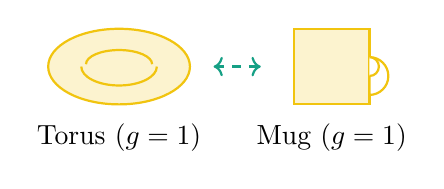
\begin{tikzpicture}[scale=0.6]
        % 甜甜圈 (Torus)
        \draw[thick, headerblue, fill=headerblue!20] (0,0) ellipse (1.5 and 0.8);
        \draw[thick, headerblue] (-0.8,0) arc (180:360:0.8 and 0.4);
        \draw[thick, headerblue] (-0.7,0.05) arc (180:0:0.7 and 0.3);
        \node[below] at (0,-1) {Torus ($g=1$)};
        
        % 箭头
        \draw[<->, thick, section2, dashed] (2,0) -- (3,0);
        
        % 咖啡杯 (Mug) - 简化画法
        \begin{scope}[xshift=4.5cm]
            \draw[thick, headerblue, fill=headerblue!20] (-0.8, -0.8) rectangle (0.8, 0.8);
            \draw[thick, headerblue, fill=white] (0.8, 0.2) arc (90:-90:0.4) -- cycle; % 把手
            \draw[thick, headerblue, fill=white] (0.8, 0.2) arc (90:-90:0.2); % 把手孔
            \node[below] at (0,-1) {Mug ($g=1$)};
        \end{scope}
    \end{tikzpicture}
    \end{center}

    \hspace{1em}拓扑学是\textbf{橡皮泥几何学}。它不关心长度、角度、面积,只关心\textbf{洞}的个数和\textbf{连通性}。
    \vspace{4pt}
    
    \subt{三大核心视角}
    \begin{itemize}[itemsep=4pt]
        \item \textbf{连续形变}: 
        只要不撕破、不粘合,物体就是一样的 (同胚)。在拓扑学家眼里,正方体和球体是一样的,但和圆环不一样。
        
        \item \textbf{局部与全局}: 
        流形在局部都是平的 (欧几里得),但全局可能有洞、扭曲 (莫比乌斯带)。代数拓扑就是用代数工具 (群) 来探测这些全局特征。
        
        \item \textbf{降维打击}: 
        欧拉示性数 $\chi$ 把复杂的几何形状压缩成了一个整数。这是数学抽象的极致体现。
    \end{itemize}
    
    \vspace{6pt}
    \centering\textit{\footnotesize 洞,定义了实体的本质。}
\end{mybox}

\end{multicols*}

\end{document}
